\documentclass[a4paper,11pt,twocolumn]{article}
\usepackage[top=1.2in, bottom=1in, left=1.4in, right=1.4in]{geometry}
\usepackage{algorithmic}
\usepackage{graphicx}
\usepackage{float}
\graphicspath{ {images/} }
\usepackage{algorithm}
\title{Single and Multiple Pattern String Matching
Algorithm \\ {\normalsize Course Project of CS4040 Bio Informatics \\Final Report}}\author{Ammanamanchi Sai Karthik, Basireddy Praveen Kumar Reddy }
\begin{document}
\maketitle
\abstract{}\textbf{Background/Objectives:} Information Retrieval Systems (IRS) are playing an eminent role in different applications like
World Wide Web, DNA sequence retrieval, etc. Basically, the IRS systems use the string matching algorithms.\\
 \textbf{Methods/
Statistical Analysis:} Since IRS uses string matching algorithms. If string matching algorithms quality is improved then
automatically information retrieval system will achieve the most relevant results. For this retrieval purpose in this paper,
single pattern and multiple pattern string matching algorithms are proposed.\\
 \textbf{Findings:} To assess the efficiency of the
proposed single pattern and multiple pattern string matching algorithm in this paper, DNA sequences of different monkeys
datasets called Pan paniscus (2.71 Gb) are considered and different tetra patterns TAGA, TCTG are searched in this
data sets. From the experimental results, it is observed that proposed single pattern and multiple pattern string matching
algorithms outperforms compared to other well-known string matching algorithms.\\
 \textbf{Application/Improvements:} It is
also observed that multiple pattern string matching algorithm reduces search time and unnecessary comparisons when
compared to single pattern string matching and other existing string matching algorithms. These proposed algorithms
very useful when we searching about the multiple patterns.
\section{Introduction}
String matching is the process of searching for the occurrence
of a specified pattern in a given text. It is one of
the important aspects of many applications as said in the
abstract. It is divided into single pattern and multiple patterns
groups.\\
In many information retrieval applications it is necessary to be able to locate quickly some or all occurrences of user-specified patterns of words and
phrases in text. This paper describes a simple, efficient
algorithm to locate all occurrences of any of a finite
number of keywords and phrases in an arbitrary text
string.

\section{Problem Statement}
To improve the running times of standard single and multiple string matching algorithms.\\

Single pattern matching using naive algorithm,finite automata and rabin karp algorithm run with a worst case time complexity of O(n*m) n=length of genomic data and m=length of the pattern.  \\

Multiple pattern matching using KMP algorithm which runs in linear time for a single pattern takes a time of O(k*(n+m)) where k=number of patterns and n=length of genomic data and m=length of the longest pattern. 

\section{Literature Survey}
\textbf{Naive algorithm} for single pattern matching considers the pattern to start at every index of the genetic sequence and executes the comparision function for the length of the pattern. This continues for all the indices of the genetic sequence.\\

\textbf{Time Complexity:} O(n*m)\\

n=length of genomic data and m=length of the longest pattern.
\\

\textbf{Finite Machine} for single pattern matching builds a finte state automata on the pattern along with the transition function. The building of the transition function is complex and takes O( m\textsuperscript{3} * no. of characters in pattern) which is high.\\

\textbf{Time Complexity:} O(m\textsuperscript{3} * c)\\

n=length of genomic data, m=length of the longest pattern, c=number of characters in text and pattern.\\

\textbf{Rabin Karp algorithm }for single pattern matching calculates the score for pattern length blocks for every index of gene sequence and compares the score modulo prime number(p) to the score of the pattern  modulo the prime number(p).\\
 
\textbf{Time Complexity: }This algorithm has an average case of O(n+m) but might run into its worst case of O(n*m).
n=length of genomic data and m=length of the longest pattern.

\subsection{Proposed Method}
\subsubsection{Single Pattern Matching Algorithm:}
\textbf{Knuth Morris Pratt:} \\Construct a longest proper suffix and prefix[lps] array for every index of pattern in O(m) time where m= length of pattern and then utilize this lps array while computing the gene sequence in such a way that on failure we do not go the start of the pattern but return to the index of previous match between the pattern and the gene sequence which is available from the lps array. This helps in restricting the time complexity to O(n+m) where n= length of the gene sequence.\\
\subsubsection{Multiple Pattern Matching Algorithm:}  
\textbf{Aho-Corasick Algorithm:} \\Consider a set of patterns {p1,p2...pn} and a gene sequence g. \\
Construct a trie for all the patterns{p1,p2...pn} and maintain a bit map{OUT} to indicate if a pattern ends at that node.\\
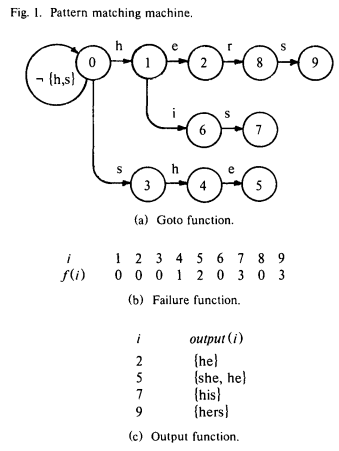
\includegraphics[scale=0.54]{trie}
Now extend the trie to a finite state automata by creating the tranisition table consisting of goto and failure transitions.\\
The goto transitions can be filled out by traversing the trie and the failure transitions can be filled out by doing a breadth first search on the trie.\\
Now the resulting finite state automata can be used for finding patterns in the gene sequence and when an accepting state is reached the corresponding patterns are obtained from the bit map{out} and the index of the pattern in gene sequence is found out. \\
This algorithm gives a time complexity of O(n+m+z) where\\
n= length of the genetic sequence\\
m= total number of characters in all patterns\\
z= total number of occurences of words indexed
\subsection{Pseudo Code}
\subsubsection{KMP algorithm:}
\begin{figure}[H]
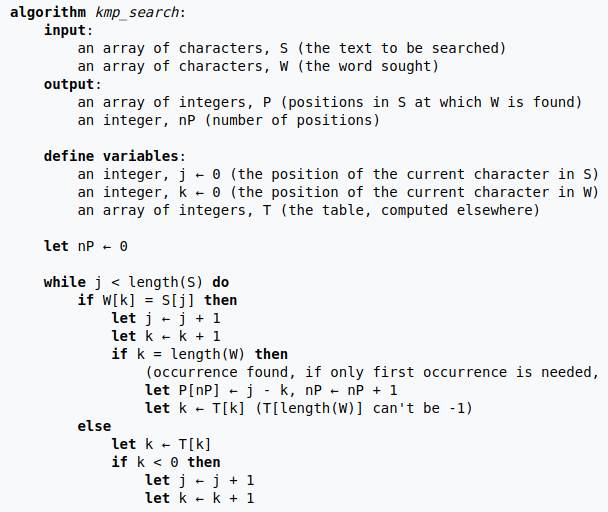
\includegraphics[width=6.8cm,height=7cm]{kmp}
\end{figure}

\begin{figure}[H]
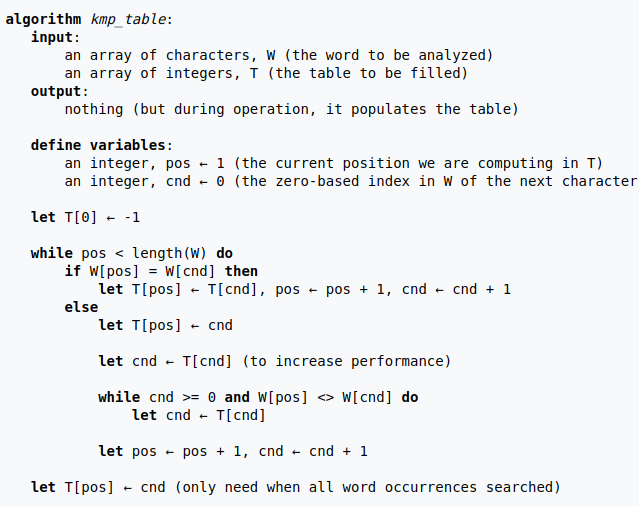
\includegraphics[width=6.8cm,height=7cm]{table}
\end{figure} 
\subsubsection{Aho-Corasick algorithm:}

\begin{figure}[H]
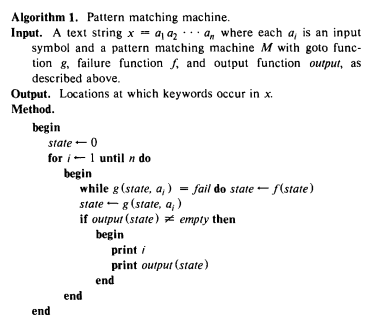
\includegraphics[width=6.8cm,height=6cm]{algo1}
\end{figure} 

\begin{figure}[H]
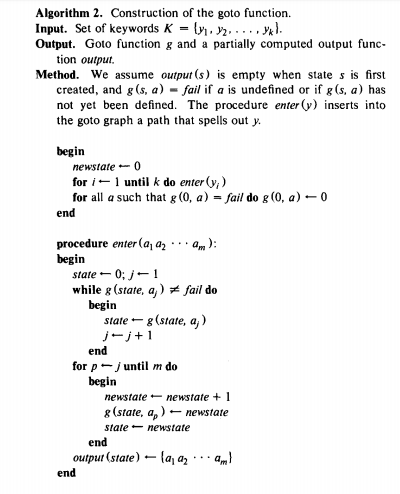
\includegraphics[width=6.8cm,height=8.5cm]{algo2}
\end{figure} 

\begin{figure}[H]
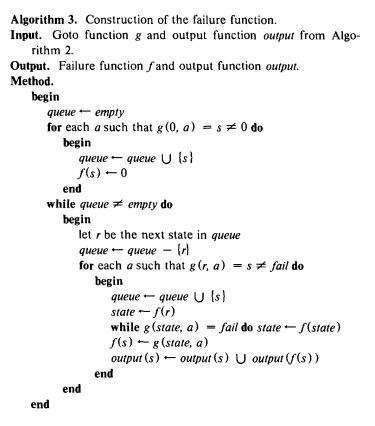
\includegraphics[width=6.8cm,height=7.5cm]{algo3}
\end{figure} 

\begin{figure}[H]
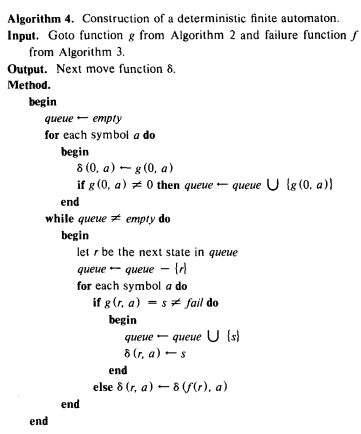
\includegraphics[width=6.8cm,height=8cm]{algo4}
\end{figure} 
\subsection{Results}
In general a monkey chromosome contains 10 (TAGA,
TCAT, GAAT, AGAT, AGAA, GATA, TATC, CTTT, TCTG
and TCTA) Complex DNA Index Structures (CODIS),
here these 10 CODIS are considered as search patterns.\\
To assess the efficiency of the proposed string matching
algorithms, all the chromosomes of  Pan paniscus (2.71 Gb are considered as data
sets.Implementation is in C++ and the program was run on Intel quad core@ 2.2Ghz and 8GB of RAM.\\
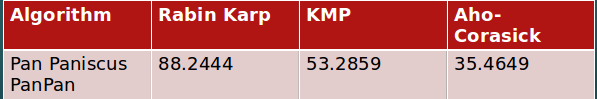
\includegraphics[width=6.8cm,height=1.8cm]{time}
\section{Conclusion}
The experimental results have shown that the single pattern string matching algorithm(KMP algorithm) reduced the search time when compared with other string matching algorithms. \\
Whereas, the multiple string matching algorithms out-perform in terms of search time as compared to proposed single pattern and existing string matching algorithms. 

\begin{thebibliography}{}
\bibitem{bib1}
 Knuth D, James H, Morris Jr, Pratt V \textit{Fast pattern matching
in strings}, SIAM Journal on Computing, 1977.
\bibitem{bib2}
Aho AV, Corasick MJ. \textit{Efficient string matching: An aid to
bibliographic search},  Communications of the ACM, 1975.
\bibitem{bib3}
Karp RM, Rabin MO. \textit{Efficient randomized pattern-matching
algorithms.},  CIBM Journal of Research and Development, 1987.
\bibitem{bib4}
Chinta Someswara Rao, K. Butchi Raju \textit{Single and Multiple Pattern String Matching Algorithm.},  Indian Journal of Science and Technology, 2016.
\end{thebibliography}{}
\end{document}

